
\title{15-440: Lab 3}
\author{
        Spencer Barton (sebarton)\\
        Emma Binns (ebinns)
}
\date{November 18, 2014}

\documentclass[12pt]{article}

\usepackage{graphicx}
\usepackage[compact]{titlesec}
\usepackage[letterpaper, portrait, margin=1in]{geometry}
\usepackage{amsmath, amsfonts, amsthm, amssymb}

\newcommand{\ttt}{\texttt}

\setlength{\parindent}{0pt}
\setlength{\parskip}{\baselineskip}

\begin{document}
\maketitle

%------------------------------------------
\pagebreak
\section{Running the Framework}

\subsection{System Requirements}

MapReduce runs on a unix cluster. The CMU unix cluster will work. Place the code in a file on AFS as we rely on that file system to share all of our code files between participants.

\subsection{Set-up}

The following steps must be followed for a successful set-up.

\begin{enumerate}
\item 
Run \ttt{python SETUP.py} in the \ttt{src} directory. This will compile all of the code.

\item
Start participants: Connect with all machines that you wish to run participants on. Run \ttt{java participant\\Participant} from the \ttt{src} directory. If this does not work you may need to use the non-default port. Try running with the optional port argument \ttt{java participant/Participant <port>}. If you see the message \ttt{File server ran into trouble} then the file server is unable to run on that machine so try running the participant on anther machine. An important note is that participants must run on different machines.

\item
Once you have some participants running, you will need to update the config file to point to these participants. Example config files can be found at \ttt{src/examples/wordcount/wordcount.config} and \ttt{src/examples/wordoccurences/wordoccurences.config}. The key lines to modify, if you plan to run the examples, are \ttt{PARTICIPANT} and \ttt{NUM\_REDUCERS}. The \ttt{PARTICIPANT} values is \ttt{<hostname>:<port>}. When you started the participants there was a message to tell you which port it is running on.

\item
You are now ready to start the master. Pick a machine that does not have a participant running on it. Run \ttt{java master/Master} from the \ttt{src} directory.

\item
The master is now running. You will have a number of possible commands to enter to run jobs. See the next section for details.

\end{enumerate}

\subsection{Manage a Job}

Now that you have the master and participants running you are ready to start a job. The master provides a command line interface to type three possible commands.

\begin{itemize}
\item
\ttt{start <path\_to\_config\_file>} This will start a process and print results as the process goes. It will also print the process id (PID) for your use with other commands.

\item
\ttt{stop <pid>} Stops the specified process

\item
\ttt{status <pid>} Gets the status of the specified process

\end{itemize}

%------------------------------------------
\section{For the Application Developer}

\subsection{Writing Your Map-Reduce Functions}

We provide two interfaces to which the application developer must adhere. The first is \ttt{MapFn} which requires a \ttt{map(String input) -> MRKeyVal(String key, int value)} method. This method takes strings which are the lines of the input file and maps them to a key-value pairs where keys are strings and values integers. If \ttt{map} returns \ttt{null} then the mapper framework will ignore the result.

The second interface is \ttt{ReduceFn} which requires a \ttt{reduce(String key, List<int> values) -> MRKeyVal(String key, int value)} method. This method takes a key and all of the values that had that key and returns a reduced result on the values in the form of a single key-value pair. If this method returns \ttt{null} then the result is ignored.

\subsection{Running Provided Examples}

To run the provided examples follow the above steps and use the provided config files. Make sure to modify the participants and number of participants as necessary. Take a look at the provided code for examples of how to write the map and reduce functions.

\subsubsection{Word Count}
Word counts takes a file of one word per line and returns the sorted words with their counts. 

Using the above steps run with \ttt{src/examples/wordcount/wordcount.config}.

The provided config file takes as input a file with all of the words in \textit{Macbeth} and outputs a word count. The only thing necessary to change in the config file is the participants and number of participants.

\subsubsection{Word Occurrences}
Word occurrences looks specifically for the word `macbeth' in the text of the play \textit{Macbeth} and returns a count of the occurrences.

Using the above steps run with \ttt{src/examples/wordoccurences/wordoccurences.config}.

The provided config file takes as input a file with all of the text of \textit{Macbeth} and outputs a word count for the word `macbeth'. The only thing necessary to change in the config file is the participants and number of participants.

\subsection{Using Remote Files}

The remote file system is abstracted away in this system. Partitions, a name for the intermediate file type used in our framework, extend the \ttt{RemoteFile}. Remote files keep track of their original machine so that when the partition reference is passed to a new machine the file itself can be brought over from the original machine. Both participants and master run a file server which serves these remote files from the `/tmp' directory. If the application developer wishes to utilize the remote file object than they can instantiate a \ttt{RemoteFile} as long as the base file lives in the `/tmp' directory.

Remote files provide a \ttt{load} method to get the file from the remote machine. This must be called before doing anything on the file.

%------------------------------------------
\section{Project Requirements}

\subsection{Requirements Met and Capabilities}

We have met all of the 

TODO UML, FLOW DIAGRAMS\\
\newpage
UML Diagram of our MapReduce facility: \\
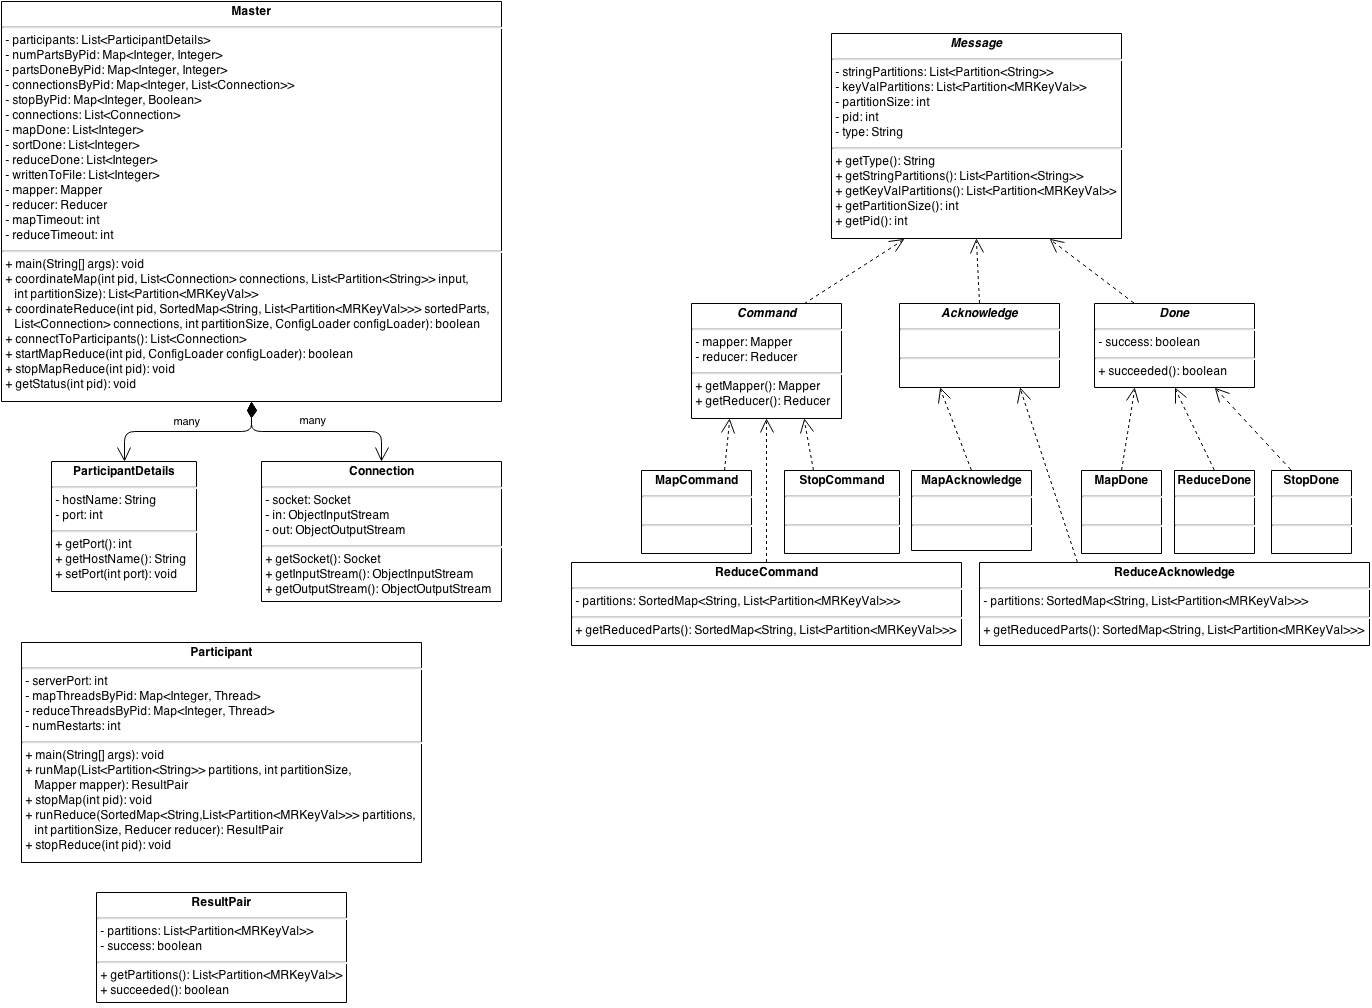
\includegraphics[scale=.35]{MapReduce_UML.png}

\newpage
Flow Diagram for user input "\verb|start <config file>|": \\
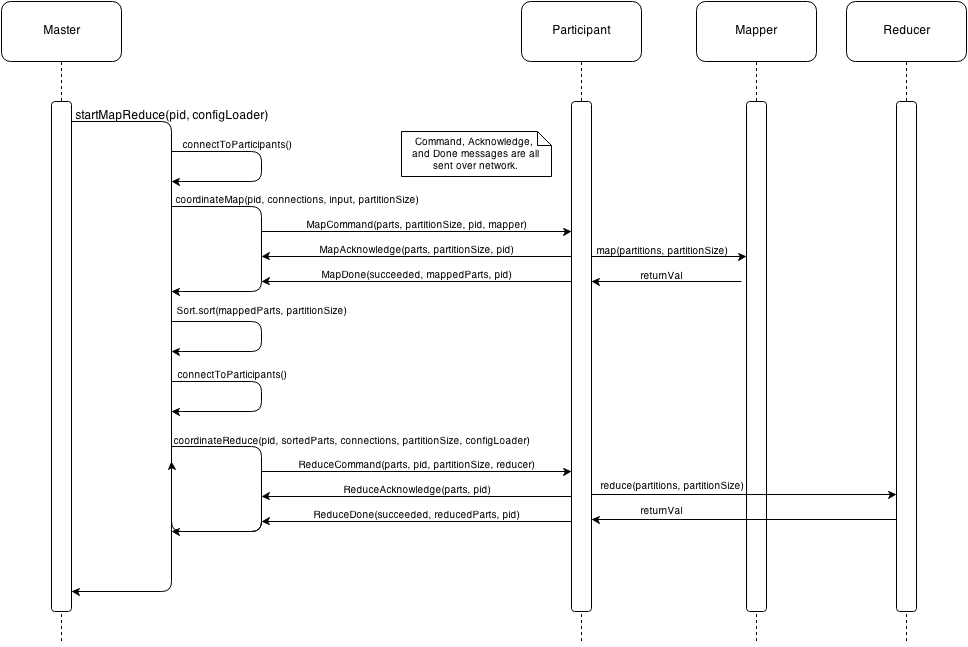
\includegraphics[scale=.5]{MapReduce_start.png}

Flow Diagram for user input "\verb|stop <pid>|": \\
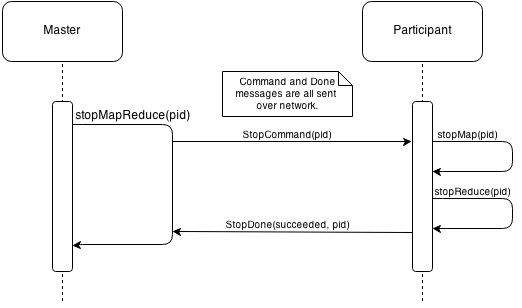
\includegraphics[scale=.7]{MapReduce_stop.png}

\subsection{Requirements Not Met and Limitations}

\subsection{Improvements}

\end{document}
